% Dit werk is gelicenseerd onder de licentie Creative Commons Naamsvermelding-GelijkDelen 4.0 Internationaal. Ga naar http://creativecommons.org/licenses/by-sa/4.0/ om een kopie van de licentie te kunnen lezen.
\documentclass[t]{beamer}

% vaak gebruikte packages, nederlands
\usepackage[margin=2.5cm]{geometry}     % Marges instellen
\usepackage[dutch]{babel}               % Voor nederlandstalige hyphenatie (woordsplitsing)
\usepackage{amsmath,amsthm}             % Uitgebreide wiskundige mogelijkheden
\usepackage{url}                        % Om url's te verwerken
\usepackage{graphicx,subfigure}         % Om figuren te kunnen verwerken
\usepackage{color}
\usepackage{framed}
\usepackage{multicol}
\usepackage[small,bf,hang]{caption}     % Om de captions wat te verbeteren
\usepackage[utf8]{inputenc}             % Om niet ascii karakters rechtstreeks te kunnen typen
\usepackage{float}                      % Om nieuwe float environments aan te maken. Ook optie H!
\usepackage{flafter}                    % Opdat floats niet zouden voorsteken
\usepackage[section]{placeins}			% Om ervoor te zorgen dat floats binnen dezelfde section blijven
\usepackage[nottoc]{tocbibind}			% Bibliografie en inhoudsopgave in ToC; zie tocbibind.dvi
\usepackage{fancyhdr}                   % Voor fancy headers en footers
\usepackage{thmtools}                   % theorem tools
\usepackage{parskip}                    % Om paragrafen met een verticale spatie ipv horizontaal te laten beginnen
\usepackage[plainpages=false]{hyperref} % Om hyperlinks te hebben in het pdfdocument.



%%%%%%%%%%%%%%%%%%%%%%%%%%%%%%
% Algemene instellingen van het document.
%%%%%%%%%%%%%%%%%%%%%%%%%%%%%%
\renewcommand{\baselinestretch}{1.2} 	% De interlinie afstand wat vergroten.
\setcounter{MaxMatrixCols}{50}          % Max 20 kolommen in een matrix


%%%%%%%%%%%%%%%%%%%%%%%%%%%%%%
% Headers en footers
%%%%%%%%%%%%%%%%%%%%%%%%%%%%%%
\pagestyle{fancy}
\fancyhf{}
\renewcommand{\headrulewidth}{0pt}
\fancyhead[RO] {\rightmark}
\fancyhead[LE] {\leftmark}
\fancyfoot[RO,LE] {\thepage}

% no dot after chapter number
\renewcommand{\chaptermark}[1]{
	\markboth{\MakeUppercase{ \chaptername\ \thechapter\quad #1}}{}
}
% no dot after section number
\renewcommand{\sectionmark}[1]{
	\markright{\MakeUppercase{ \thesection\quad #1}}{}
}

% page header and footer style in mainmatter aanpassen
\let\newmainmatter\mainmatter
\renewcommand{\mainmatter}{

	\pagestyle{fancy}
	\fancyhf{}
	\renewcommand{\headrulewidth}{0pt}
	\fancyhead[RO] {\rightmark}
	\fancyhead[LE] {\leftmark}
	\fancyfoot[RO,LE] {\thepage}
	\fancyfoot[C]{\tiny{Brecht Baeten}}

	\newmainmatter
}
\let\newappendix\appendix
\renewcommand{\appendix}{
	\fancyfoot{}
	\fancyfoot[RO,LE] {\thepage}
	\newappendix
}


%%%%%%%%%%%%%%%%%%%%%%%%%%%%%%
% Nieuwe omgevingen
%%%%%%%%%%%%%%%%%%%%%%%%%%%%%%
\definecolor{shadecolor}{gray}{0.95}
\newcounter{voorbeeldcounter}[chapter]
\renewcommand{\thevoorbeeldcounter}{\thechapter.\arabic{voorbeeldcounter}}
\makeatletter
\newenvironment{voorbeeld}
{
\vspace{3mm}
\addtolength{\leftskip}{5mm}
\begin{shaded*}
\vspace{-3mm}
\refstepcounter{voorbeeldcounter}
\noindent
\textbf{Voorbeeld \thevoorbeeldcounter:\\}
%\vspace{-8mm}
%\begin{multicols}{2}
}
{
%\end{multicols}
\end{shaded*}
\addtolength{\leftskip}{-5mm}
}
\makeatother  
    
%%%%%%%%%%%%%%%%%%%%%%%%%%%%%%
% .svg commando's
%%%%%%%%%%%%%%%%%%%%%%%%%%%%%%
% nieuw commando om svg files dynamisch te updaten
%\newcommand{\executeiffilenewer}[3]{%
%\ifnum\pdfstrcmp{\pdffilemoddate{#1}}%
%{\pdffilemoddate{#2}}>0%
%{\immediate\write18{#3}}\fi%
%}
%% nieuw commando om. svg figuren in te voegen
%% Gebruik: \includesvg{path/filename.svg}
%\newcommand{\includesvg}[2][0]{%
%\executeiffilenewer{#2.svg}{#2.pdf}%
%{inkscape -z -C --file=#2.svg %
%--export-pdf=#2.pdf --export-latex}%
%\ifx#10
%	\let\svgwidth\undefined
%\else
%	\def\svgwidth{#1}
%\fi%
%\input{#2.pdf_tex}%
%\ifx \svgwidth\undefined
%\else
%	\let\svgwidth\undefined
%\fi%
%}

% nieuw commando om .fig figuren in te voegen
\newcommand{\includefig}[2][0]{%
\ifx#10
	\let\figwidth\undefined
\else
	\def\figwidth{#1}
\fi%
\input{#2.pdf_tex}%
\ifx \figwidth\undefined
\else
	\let\figwidth\undefined
\fi%
}

%%%%%%%%%%%%%%%%%%%%%%%%%%%%%%
% Packages
%%%%%%%%%%%%%%%%%%%%%%%%%%%%%%

%\usepackage{geometry}              	% 
\usepackage[dutch]{babel}               % Voor nederlandstalige hyphenatie (woordsplitsing)
\uselanguage{dutch}
\languagepath{dutch}
\usepackage{amsmath,amsthm}             % Uitgebreide wiskundige mogelijkheden
\usepackage{url}                        % Om url's te verwerken
\usepackage{graphicx,subfigure}         % Om figuren te kunnen verwerken
\usepackage[utf8]{inputenc}             % Om niet ascii karakters rechtstreeks te kunnen typen
\usepackage[section]{placeins}			% Om ervoor te zorgen dat floats binnen dezelfde section blijven
\usepackage{multicol}
\usepackage[absolute,overlay]{textpos}

%%%%%%%%%%%%%%%%%%%%%%%%%%%%%%
% Layout
%%%%%%%%%%%%%%%%%%%%%%%%%%%%%%
\usetheme{Frankfurt}
\usefonttheme[onlymath]{serif}
\AtBeginSection[]
{
  \begin{frame}
    \frametitle{Inhoud}
    \tableofcontents[currentsection]
  \end{frame}
}

\setbeamertemplate{navigation symbols}{}
\setbeamertemplate{footline}[page number]

%%%%%%%%%%%%%%%%%%%%%%%%%%%%%%
% Title
%%%%%%%%%%%%%%%%%%%%%%%%%%%%%%
\title{Fluïdummechanica}
\author{Brecht Baeten\inst{1}}
\institute{
	\inst{1}%
  		KU Leuven, Technologie campus Diepenbeek,\\ e-mail: brecht.baeten@kuleuven.be
}
\date{\today}
%%%%%%%%%%%%%%%%%%%%%%%%%%%%%%
% Omgevingen
%%%%%%%%%%%%%%%%%%%%%%%%%%%%%%


\subtitle{Leidingstelsels}

\begin{document}

	\frame{\titlepage}
%%%%%%%%%%%%%%%%%%%%%%%%%%%%%%%%%%%%%%%%%%%%%%%%%%%%%%%%%%%%%%%%%%%%%%%%%%%
	\section{Inleiding}
	\begin{frame}
		\frametitle{Voorbeeld}
		\center
    	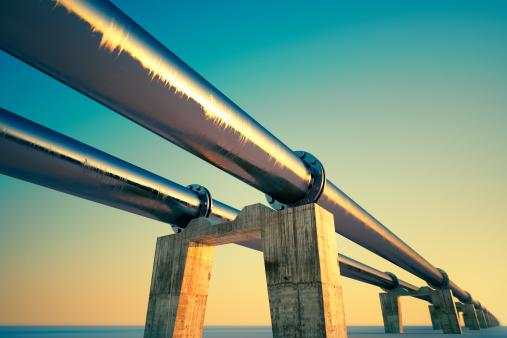
\includegraphics[width=\textwidth]{fig/stroming_in_leidingen/Richard-Steinberg-The-Pipeline-Blog-51.jpg}\\
    	\footnotesize{Bron: http://www.etftrends.com/}
  	\end{frame}
%%%%%%%%%%%%%%%%%%%%%%%%%%%%%%%%%%%%%%%%%%%%%%%%%%%%%%%%%%%%%%%%%%%%%%%%%%%
  	\section{Mechanische energie}
  	\begin{frame}
		\frametitle{Bernoulli}
		\only<1-4>{
			Behoud van mechanisch energie:
			\begin{equation*}
				p_2 + \rho \frac{1}{2} v_2^2 + \rho g z_2 = p_1 + \rho \frac{1}{2} v_1^2 + \rho g z_1
			\end{equation*}
		}
		\only<2-4>{
			Door viskeuze wrijving wordt een gedeelte van de mechanische energie gedissipeerd:
			\begin{equation*}
				p_2 + \rho \frac{1}{2} v_2^2 + \rho g z_2 = p_1 + \rho \frac{1}{2} v_1^2 + \rho g z_1 - \Delta E
			\end{equation*}
		}
		\only<3-4>{
			Voor een rechte horizontale cilindrische leiding:
			\begin{equation*}
				\Delta E = p_1 - p_2  
			\end{equation*}	
		}
		\only<4-4>{
			\begin{equation*}
				\Delta E = f \frac{1}{2} \rho v^2 \frac{L}{D}
			\end{equation*}
		}
	\end{frame}
%%%%%%%%%%%%%%%%%%%%%%%%%%%%%%%%%%%%%%%%%%%%%%%%%%%%%%%%%%%%%%%%%%%%%%%%%%%
  	\begin{frame}
		\frametitle{Ladingsverlies}
		\only<1-3>{
			Stel de vergelijking voor mechanische energie voor in eenheid hoogte:
			\begin{equation}
				\frac{p_2}{\rho g} + \frac{v_2^2}{2 g} + z_2 = \frac{p_1}{\rho g} + \frac{v_1^2}{2 g} + z_1 - h_L
			\end{equation}		
		}
		\only<2-3>{
			Ladingsverlies voor een cilindrische leiding:
			\begin{equation}
				h_\mathrm{L} = f \frac{v^2}{2 g} \frac{L}{D}
			\end{equation}
		}
		\only<3-3>{
			\begin{equation}
				h_\mathrm{L} = 8 f \frac{\dot{V}^2}{g \pi^2} \frac{L}{D^5}
			\end{equation}
		}
	\end{frame}
%%%%%%%%%%%%%%%%%%%%%%%%%%%%%%%%%%%%%%%%%%%%%%%%%%%%%%%%%%%%%%%%%%%%%%%%%%%
  	\begin{frame}
		\frametitle{Grafische voorstelling}
		
	\end{frame}
%%%%%%%%%%%%%%%%%%%%%%%%%%%%%%%%%%%%%%%%%%%%%%%%%%%%%%%%%%%%%%%%%%%%%%%%%%%
  	\section{Lokale ladingsverliezen}
  	\begin{frame}
		\frametitle{Voorbeelden}
		\center
		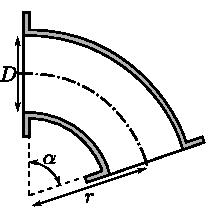
\includegraphics[width=0.3\textwidth]{fig/appendix/Bocht} \quad
		\includegraphics[width=0.3\textwidth]{fig/appendix/Gelijkdelijke_vernauwing} \quad
		\includegraphics[width=0.3\textwidth]{fig/appendix/Gelijkdelijke_verwijding}
		\\
		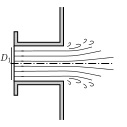
\includegraphics[width=0.3\textwidth]{fig/appendix/Uitstroming} \quad
		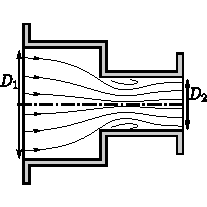
\includegraphics[width=0.3\textwidth]{fig/appendix/Vernauwing} \quad
		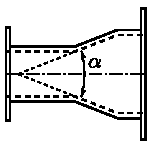
\includegraphics[width=0.3\textwidth]{fig/appendix/Verwijding}
	\end{frame}
%%%%%%%%%%%%%%%%%%%%%%%%%%%%%%%%%%%%%%%%%%%%%%%%%%%%%%%%%%%%%%%%%%%%%%%%%%%
  	\begin{frame}
		\frametitle{Verliescoëfficient}	
		\only<1-3>{
			\center
			Lokale ladings verliezen kunnen in rekening gebracht worden met behulp van een empirisch bepaalde verliescoëfficient $\zeta$
		}
		
		\only<2-3>{
			\begin{equation*}
				h_\mathrm{L,lokaal} = \zeta \frac{v^2}{2 g}
			\end{equation*}
		}
		\only<3-3>{
			\begin{equation*}
				h_\mathrm{L,lokaal} = \zeta \frac{\dot{V}^2}{2 g A^2}
			\end{equation*}
		}
		
	\end{frame}
%%%%%%%%%%%%%%%%%%%%%%%%%%%%%%%%%%%%%%%%%%%%%%%%%%%%%%%%%%%%%%%%%%%%%%%%%%%
  	\begin{frame}
		\frametitle{Plotse Verwijding}
		\only<1>{
			\center
			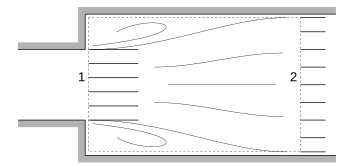
\includegraphics[width=\textwidth]{fig/leidingstelsels/Plotse_verwijding}
		}
		\only<2-5>{
			\begin{textblock}{5}(0,3)
            	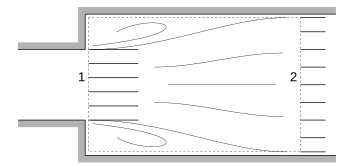
\includegraphics[width=5cm]{fig/leidingstelsels/Plotse_verwijding}
       		\end{textblock}
       		\vspace{2.5cm}
		}
		\only<2-5>{
			\begin{equation*}
				p_1 A_2 - p_2 A_2 = \rho A_2 v_2 (v_2-v_1)
			\end{equation*}
		}
		\only<3-5>{
			\begin{equation*}
				\frac{p_2}{\rho g} + \frac{v_2^2}{2 g} = \frac{p_1}{\rho g} + \frac{v_1^2}{2 g} - h_L
			\end{equation*}
		}
		\only<4-5>{
			\begin{equation*}
				h_L = \frac{v_1^2}{2 g} \left(1 - 2\frac{v_2}{v_1} + \frac{v_2^2}{v_1^2} \right)
			\end{equation*}
		}
		\only<5-5>{
			\begin{equation*}
				h_L = \frac{v_1^2}{2 g} \left(1 - \frac{A_1}{A_2} \right)^2
			\end{equation*}
		}
	\end{frame}
%%%%%%%%%%%%%%%%%%%%%%%%%%%%%%%%%%%%%%%%%%%%%%%%%%%%%%%%%%%%%%%%%%%%%%%%%%%
  	\begin{frame}
		\frametitle{Voorbeeld van empirische data}
		\center
		\begin{tabular}{p{7cm} p{3cm}}
			\vtop{\null\hbox{
				\begin{tabular}{l c c c c c}
					$r/D$        & 1    & 2    & 4    & 6    & 10   \\
					\hline
					$\zeta$ glad & 0.21 & 0.14 & 0.11 & 0.09 & 0.11 \\
					$\zeta$ ruw  & 0.51 & 0.30 & 0.23 & 0.18 & 0.20 \\
				\end{tabular}
			}}
			&
			\vtop{\null\hbox{
				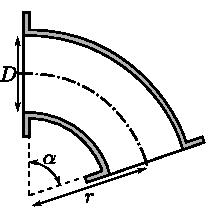
\includegraphics[width=3cm]{fig/appendix/Bocht}
			}}
		\end{tabular}
		
		\center
		Het totale ladingsverlies is steeds het lokale verlies plus het verlies ten gevolge van de lengte van de leiding.
	
	\end{frame}
%%%%%%%%%%%%%%%%%%%%%%%%%%%%%%%%%%%%%%%%%%%%%%%%%%%%%%%%%%%%%%%%%%%%%%%%%%%	
	\begin{frame}
		\frametitle{Voorbeelden}
		\center
		\includegraphics[height=0.8\textheight]{fig/appendix/verwijding}
	\end{frame}
%%%%%%%%%%%%%%%%%%%%%%%%%%%%%%%%%%%%%%%%%%%%%%%%%%%%%%%%%%%%%%%%%%%%%%%%%%%	
	\begin{frame}
		\frametitle{Voorbeelden}
		\center
		\includegraphics[height=0.8\textheight]{fig/appendix/gelijkdelijke_verwijding}
	\end{frame}
%%%%%%%%%%%%%%%%%%%%%%%%%%%%%%%%%%%%%%%%%%%%%%%%%%%%%%%%%%%%%%%%%%%%%%%%%%%	
	\begin{frame}
		\frametitle{Voorbeelden}
		\center
		\includegraphics[height=0.8\textheight]{fig/appendix/uitstroming}
	\end{frame}
%%%%%%%%%%%%%%%%%%%%%%%%%%%%%%%%%%%%%%%%%%%%%%%%%%%%%%%%%%%%%%%%%%%%%%%%%%%	
	\begin{frame}
		\frametitle{Voorbeelden}
		\center
		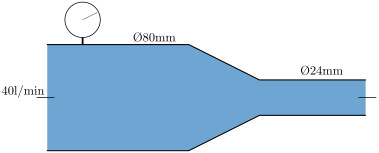
\includegraphics[height=0.8\textheight]{fig/appendix/vernauwing}
	\end{frame}
%%%%%%%%%%%%%%%%%%%%%%%%%%%%%%%%%%%%%%%%%%%%%%%%%%%%%%%%%%%%%%%%%%%%%%%%%%%	
	\begin{frame}
		\frametitle{Voorbeelden}
		\center
		\includegraphics[height=0.8\textheight]{fig/appendix/gelijkdelijke_vernauwing}
	\end{frame}	
%%%%%%%%%%%%%%%%%%%%%%%%%%%%%%%%%%%%%%%%%%%%%%%%%%%%%%%%%%%%%%%%%%%%%%%%%%%	
	\begin{frame}
		\frametitle{Voorbeelden}
		\center
		\includegraphics[height=0.8\textheight]{fig/appendix/instroming}
	\end{frame}	
%%%%%%%%%%%%%%%%%%%%%%%%%%%%%%%%%%%%%%%%%%%%%%%%%%%%%%%%%%%%%%%%%%%%%%%%%%%	
	\begin{frame}
		\frametitle{Voorbeelden}
		\center
		\includegraphics[height=0.8\textheight]{fig/appendix/afgeronde_instroming}
	\end{frame}	
%%%%%%%%%%%%%%%%%%%%%%%%%%%%%%%%%%%%%%%%%%%%%%%%%%%%%%%%%%%%%%%%%%%%%%%%%%%
  	\section{Serie en parallel schakeling}
  	\begin{frame}
		\frametitle{Serieschakeling}
		\only<1-3>{
			\center
			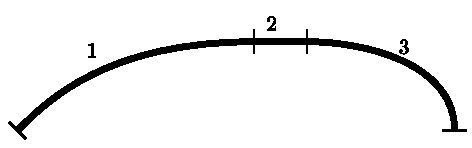
\includegraphics[width=0.8\textwidth]{fig/leidingstelsels/serieschakeling}
		}
		\only<2-3>{	
			\begin{align*}
				\dot{V}_\mathrm{serie} &= \dot{V}_i \\
				h_\mathrm{L,serie} &= \sum h_\mathrm{L,i}
			\end{align*}
		}
		\only<3-3>{
			\center
			Het totale ladingsverlies in een serieschakeling van elementen is de som van de ladingsverliezen
		}
	\end{frame}
%%%%%%%%%%%%%%%%%%%%%%%%%%%%%%%%%%%%%%%%%%%%%%%%%%%%%%%%%%%%%%%%%%%%%%%%%%%
  	\begin{frame}
		\frametitle{Parallelschakeling}
		\only<1-3>{
			\center
			\includegraphics[width=0.8\textwidth]{fig/leidingstelsels/parallelschakeling}
		}
		\only<2-3>{	
			\begin{align*}
				\dot{V}_\mathrm{parallel} &= \sum \dot{V}_i \\
				h_\mathrm{L,parallel} &= h_\mathrm{L,i}
			\end{align*}
		}
		\only<3-3>{
			\center
			Het ladingsverlies in elke tak van een parallelschakeling is gelijk aan het totale ladingsverlies
		}
	\end{frame}
%%%%%%%%%%%%%%%%%%%%%%%%%%%%%%%%%%%%%%%%%%%%%%%%%%%%%%%%%%%%%%%%%%%%%%%%%%%
\end{document}